% Options for packages loaded elsewhere
% Options for packages loaded elsewhere
\PassOptionsToPackage{unicode}{hyperref}
\PassOptionsToPackage{hyphens}{url}
\PassOptionsToPackage{dvipsnames,svgnames,x11names}{xcolor}
%
\documentclass[
  sn-basic,
]{sn-jnl}


\usepackage{xcolor}
\usepackage{amsmath,amssymb}
\setcounter{secnumdepth}{5}
\usepackage{iftex}
\ifPDFTeX
  \usepackage[T1]{fontenc}
  \usepackage[utf8]{inputenc}
  \usepackage{textcomp} % provide euro and other symbols
\else % if luatex or xetex
  \usepackage{unicode-math} % this also loads fontspec
  \defaultfontfeatures{Scale=MatchLowercase}
  \defaultfontfeatures[\rmfamily]{Ligatures=TeX,Scale=1}
\fi
\usepackage{lmodern}
\ifPDFTeX\else
  % xetex/luatex font selection
\fi
% Use upquote if available, for straight quotes in verbatim environments
\IfFileExists{upquote.sty}{\usepackage{upquote}}{}
\IfFileExists{microtype.sty}{% use microtype if available
  \usepackage[]{microtype}
  \UseMicrotypeSet[protrusion]{basicmath} % disable protrusion for tt fonts
}{}
\makeatletter
\@ifundefined{KOMAClassName}{% if non-KOMA class
  \IfFileExists{parskip.sty}{%
    \usepackage{parskip}
  }{% else
    \setlength{\parindent}{0pt}
    \setlength{\parskip}{6pt plus 2pt minus 1pt}}
}{% if KOMA class
  \KOMAoptions{parskip=half}}
\makeatother
% Make \paragraph and \subparagraph free-standing
\makeatletter
\ifx\paragraph\undefined\else
  \let\oldparagraph\paragraph
  \renewcommand{\paragraph}{
    \@ifstar
      \xxxParagraphStar
      \xxxParagraphNoStar
  }
  \newcommand{\xxxParagraphStar}[1]{\oldparagraph*{#1}\mbox{}}
  \newcommand{\xxxParagraphNoStar}[1]{\oldparagraph{#1}\mbox{}}
\fi
\ifx\subparagraph\undefined\else
  \let\oldsubparagraph\subparagraph
  \renewcommand{\subparagraph}{
    \@ifstar
      \xxxSubParagraphStar
      \xxxSubParagraphNoStar
  }
  \newcommand{\xxxSubParagraphStar}[1]{\oldsubparagraph*{#1}\mbox{}}
  \newcommand{\xxxSubParagraphNoStar}[1]{\oldsubparagraph{#1}\mbox{}}
\fi
\makeatother


\usepackage{longtable,booktabs,array}
\newcounter{none} % for unnumbered tables
\usepackage{calc} % for calculating minipage widths
% Correct order of tables after \paragraph or \subparagraph
\usepackage{etoolbox}
\makeatletter
\patchcmd\longtable{\par}{\if@noskipsec\mbox{}\fi\par}{}{}
\makeatother
% Allow footnotes in longtable head/foot
\IfFileExists{footnotehyper.sty}{\usepackage{footnotehyper}}{\usepackage{footnote}}
\makesavenoteenv{longtable}
\usepackage{graphicx}
\makeatletter
\newsavebox\pandoc@box
\newcommand*\pandocbounded[1]{% scales image to fit in text height/width
  \sbox\pandoc@box{#1}%
  \Gscale@div\@tempa{\textheight}{\dimexpr\ht\pandoc@box+\dp\pandoc@box\relax}%
  \Gscale@div\@tempb{\linewidth}{\wd\pandoc@box}%
  \ifdim\@tempb\p@<\@tempa\p@\let\@tempa\@tempb\fi% select the smaller of both
  \ifdim\@tempa\p@<\p@\scalebox{\@tempa}{\usebox\pandoc@box}%
  \else\usebox{\pandoc@box}%
  \fi%
}
% Set default figure placement to htbp
\def\fps@figure{htbp}
\makeatother


% definitions for citeproc citations
\NewDocumentCommand\citeproctext{}{}
\NewDocumentCommand\citeproc{mm}{%
  \begingroup\def\citeproctext{#2}\cite{#1}\endgroup}
\makeatletter
 % allow citations to break across lines
 \let\@cite@ofmt\@firstofone
 % avoid brackets around text for \cite:
 \def\@biblabel#1{}
 \def\@cite#1#2{{#1\if@tempswa , #2\fi}}
\makeatother
\newlength{\cslhangindent}
\setlength{\cslhangindent}{1.5em}
\newlength{\csllabelwidth}
\setlength{\csllabelwidth}{3em}
\newenvironment{CSLReferences}[2] % #1 hanging-indent, #2 entry-spacing
 {\begin{list}{}{%
  \setlength{\itemindent}{0pt}
  \setlength{\leftmargin}{0pt}
  \setlength{\parsep}{0pt}
  % turn on hanging indent if param 1 is 1
  \ifodd #1
   \setlength{\leftmargin}{\cslhangindent}
   \setlength{\itemindent}{-1\cslhangindent}
  \fi
  % set entry spacing
  \setlength{\itemsep}{#2\baselineskip}}}
 {\end{list}}
\usepackage{calc}
\newcommand{\CSLBlock}[1]{\hfill\break\parbox[t]{\linewidth}{\strut\ignorespaces#1\strut}}
\newcommand{\CSLLeftMargin}[1]{\parbox[t]{\csllabelwidth}{\strut#1\strut}}
\newcommand{\CSLRightInline}[1]{\parbox[t]{\linewidth - \csllabelwidth}{\strut#1\strut}}
\newcommand{\CSLIndent}[1]{\hspace{\cslhangindent}#1}



\setlength{\emergencystretch}{3em} % prevent overfull lines

\providecommand{\tightlist}{%
  \setlength{\itemsep}{0pt}\setlength{\parskip}{0pt}}





%%%% Standard Packages

\usepackage{graphicx}%
\usepackage{multirow}%
\usepackage{amsmath,amssymb,amsfonts}%
\usepackage{amsthm}%
\usepackage{mathrsfs}%
\usepackage[title]{appendix}%
\usepackage{xcolor}%
\usepackage{textcomp}%
\usepackage{manyfoot}%
\usepackage{booktabs}%
\usepackage{algorithm}%
\usepackage{algorithmicx}%
\usepackage{algpseudocode}%
\usepackage{listings}%

%%%%

\raggedbottom
\usepackage{booktabs}
\usepackage{longtable}
\usepackage{array}
\usepackage{multirow}
\usepackage{wrapfig}
\usepackage{float}
\usepackage{colortbl}
\usepackage{pdflscape}
\usepackage{tabu}
\usepackage{threeparttable}
\usepackage{threeparttablex}
\usepackage[normalem]{ulem}
\usepackage{makecell}
\usepackage{xcolor}
\usepackage{caption}
\usepackage{anyfontsize}
\makeatletter
\@ifpackageloaded{caption}{}{\usepackage{caption}}
\AtBeginDocument{%
\ifdefined\contentsname
  \renewcommand*\contentsname{Table of contents}
\else
  \newcommand\contentsname{Table of contents}
\fi
\ifdefined\listfigurename
  \renewcommand*\listfigurename{List of Figures}
\else
  \newcommand\listfigurename{List of Figures}
\fi
\ifdefined\listtablename
  \renewcommand*\listtablename{List of Tables}
\else
  \newcommand\listtablename{List of Tables}
\fi
\ifdefined\figurename
  \renewcommand*\figurename{Figure}
\else
  \newcommand\figurename{Figure}
\fi
\ifdefined\tablename
  \renewcommand*\tablename{Table}
\else
  \newcommand\tablename{Table}
\fi
}
\@ifpackageloaded{float}{}{\usepackage{float}}
\floatstyle{ruled}
\@ifundefined{c@chapter}{\newfloat{codelisting}{h}{lop}}{\newfloat{codelisting}{h}{lop}[chapter]}
\floatname{codelisting}{Listing}
\newcommand*\listoflistings{\listof{codelisting}{List of Listings}}
\makeatother
\makeatletter
\makeatother
\makeatletter
\@ifpackageloaded{caption}{}{\usepackage{caption}}
\@ifpackageloaded{subcaption}{}{\usepackage{subcaption}}
\makeatother
\usepackage{bookmark}
\IfFileExists{xurl.sty}{\usepackage{xurl}}{} % add URL line breaks if available
\urlstyle{same}
\hypersetup{
  pdftitle={Phoenix public parks serve as tree refuges in deprived areas},
  pdfauthor={Sean Whitcomb},
  pdfkeywords={urban forest, green space equity},
  colorlinks=true,
  linkcolor={blue},
  filecolor={Maroon},
  citecolor={Blue},
  urlcolor={Blue},
  pdfcreator={LaTeX via pandoc}}


\title[Phoenix public parks serve as tree refuges in deprived
areas]{Phoenix public parks serve as tree refuges in deprived areas}

% author setup
\author*[1]{\fnm{Sean} \sur{Whitcomb}}\email{sean.whitcomb@mesacc.edu}
% affil setup
\affil[1]{, \orgname{Mesa Community College}}

% abstract 


% keywords
\keywords{urban forest,  green space equity}

\begin{document}
\maketitle


\section{Introduction}\label{sec-introduction}

Urban trees, whether in private yards, planted along streets, or in
public parks, are a critical component of sustainable cities. The urban
forest provides numerous ecosystem services that benefit city residents,
including shade, stormwater removal, and air pollution mitigation
(CITE). Tree canopy cover (TCC), defined as the area of ground covered
by tree leaves, stems, and branches, is especially crucial in hot arid
cities like Phoenix, Arizona, where shaded ground can be up to XX C
cooler than bare ground (CITE). Adequate shade can be a lifesaving
amenity in Phoenix, which experienced XXX heat-related deaths in 2025
(CITE).

Like many urban amenities, tree canopy cover is often not equitably
distributed across cities. Several studies have shown that residents of
lower socioeconomic status tend to live in ``tree deserts,'' or
neighborhoods with lower TCC (CITE). Some studies also report that
neighborhoods with larger populations of ethnic and racial minorities
are more likely to be tree deserts (CITE). Wang, et al.~(2024)
demonstrated that these patterns hold true in Phoenix as well, finding a
positive association between TCC and median household income, a negative
correlation between TCC and percent Black population, and a negative
correlation between TCC and percent Hispanic population at the block
group level {[}1{]}.

As a source of publicly available tree canopy cover, municipal parks
could potentially act as ``tree oases'' and compensate for the lack of
tree cover in disadvantaged neighborhoods. However, numerous studies
have shown that public parks also tend to be inequitably distributed
across cities (CITE). Public parks in XXX and XXX are more concentrated
in more affluent neighborhoods with larger White populations, but the
evidence for park inequities in Phoenix is mixed. Lara-Valencia (2018)
found that Hispanic residents of Phoenix tend to have greater access to
municipal parks due to a higher concentration of parks in the urban core
{[}2{]}. However, Ibes (2015) analyzed access to public parks in Phoenix
by type of park and found that ``green neighborhood parks'' are more
concentrated in neighborhoods with higher White populations while
``urban core parks'' are more often found in areas with lower incomes
and more minority residents {[}3{]}. Corley (2024) found no association
between park acreage and minority status or poverty level at the block
group level in Phoenix {[}4{]}. The previously mentioned studies on
Phoenix park access did not account for spatial autocorrelation of
variables, i.e, observations that are spatially proximate tend to be
more similar than expected under random distribution (CITE). When Kim,
et al.~(2023) used spatial regressive models to investigate park access
in Phoenix and nearby Mesa, AZ, they found that more affluent
neighborhoods had access to greater park acreage within walking
distance, but there were no significant correlations between
race/ethnicity of residents and the number of parks, size of parks, or
distance to the nearest park {[}5{]}.

All of the aforementioned studies on Phoenix-area parks have used a
simple Euclidean distance metric to determine ``access,'' but this
method does not account for the actual distance that residents must
travel to visit the parks. The travel distance from a home to a public
amenity can vary greatly from the Euclidean distance depending on the
layout of the road network (CITE). Most studies consider ``park access''
to be a binary variable, where a resident has complete access to any
parks within a given catchment area and no access to parks outside of
the catchment area. However, this approach does not capture the reality
of park visitation--people are more likely to visit nearby parks, but
will still travel a greater distance to visit larger parks. Kim et
al.~(2023) found that Phoenix residents tend to favor local parks within
1 km of their neighborhood, but the likelihood that they will travel
beyond 1 km to visit larger amenity-rich parks increases as the size of
the local parks decreases {[}6{]}. Traditional park access research also
tends to only address the ``supply'' side of access by quantifying park
number, area, or amenities (CITE) and ignoring the ``demand'' side, or
the number of people competing for access to the parks. Other studies
incorporate the population factor by simply dividing the total park area
by the population within a given catchment {[}7{]} (CITE MORE?). The
Gaussian two-step floating catchment area (G2SFCA) method addresses
these shortcomings by incorporating a park supply factor (e.g., total
area or amenities), a demand factor (the population of residents with
access to the parks), and a travel distance metric that weights closer
parks more heavily than distant parks {[}8{]}.

An accurate assessment of park access using the G2SFCA method depends on
the choice of supply and demand origin points used to determine travel
distance from residents to parks. Census block group centroids are often
used as demand origin points because they represent the ``average''
location of residents within a reasonably small area (CITE). However,
population-weighted block group centroids are less likely to
underestimate accessibility {[}9{]}. For example, the geographic
centroid of a large block group with housing concentrated in one small
corner is likely to be located far from areas where most people live,
leading to a suboptimal estimate of the travel distance to a public
park. Likewise, the geographic centroid of a park is commonly used as
the supply origin point, but this choice can provide an inaccurate
picture of park access, especially in large parks or long linear parks
where the centroid is far from the entrances. Residents also may not be
able to access parks at any point along the boundary but are instead
limited to a small number of entrances. Using park entrances rather than
centroids as the supply origin points in a G2SFCA analysis overcomes
these limitations {[}8{]}.

Residential tree canopy cover provided by trees in neighborhoods and
commercial areas likely has a more direct impact on residents' lives
than the tree canopy in public parks since residential trees shade
people's homes, workplaces, and travel routes. But parks may act as tree
canopy oases, allowing people to temporarily enjoy the benefits of trees
that may be lacking in their daily lives. No studies have investigated
the relationship between residential tree canopy cover and access to
park tree canopy cover, but a 2013 study by Zhou and Kim investigated
neighborhood tree canopy disparities and general walking-distance access
to parks in six Illinois cities {[}10{]}. They found that in four of the
cities, a higher proportion of Black residents was associated with lower
tree canopy cover, but there were no disparities in access to parks.
However, this study did not quantify the tree canopy cover within parks.
This is a serious limitation because parks can vary widely in size and
they may not all contain adequate tree cover to provide shade for nearby
residents.

Past research on tree canopy equity has identified tree deserts in
Phoenix neighborhoods, but no studies to date have isolated residential
tree canopy cover from public park canopy cover. There is also a lack of
research addressing whether Phoenix public parks act as tree canopy
refuges that partially compensate for lack of tree cover in the
surrounding neighborhoods. This study attempts to address these research
gaps by answering the following questions:

\begin{enumerate}
\def\labelenumi{\arabic{enumi}.}
\item
  To what extent do racial/ethnic composition and socioeconomic
  deprivation predict residential (non-park) tree canopy cover across
  Phoenix neighborhoods?
\item
  To what extent do racial/ethnic composition and socioeconomic
  deprivation predict public park tree canopy accessibility in Phoenix,
  and does this relationship diverge from the patterns observed for
  residential tree canopy?
\item
  Do Phoenix public parks function as tree canopy refuges --- i.e., do
  neighborhoods with low residential tree canopy have disproportionately
  high access to park tree canopy --- and does this compensatory pattern
  hold uniformly across racial/ethnic groups and deprivation levels?
\end{enumerate}

\section{Materials and methods}\label{sec-methods}

\subsection{Study area}\label{study-area}

The study area is the city of Phoenix in Maricopa County, Arizona, USA.
AREA\ldots{} It has a population of 1.67 million as of 2024, making it
the fifth largest city in the country {[}11{]}. The Phoenix metro area
consists of 26 municipalities with a total of 4.7 million inhabitants.
The population of Phoenix is ethnically and racially diverse. Of the
block groups included in this study, Hispanic residents make up 39.6\%
of the population, and Black residents make up 6.8\%, according to data
from the 2021-2024 5-year American Community Survey (ACS). The median
household income is \$\ensuremath{9.082259\times 10^{4}}. FIX THIS

Phoenix is located in the Sonoran Desert and has a semi-arid climate
with hot summers and mild winters. The average daily mean
temperature\ldots{}

\subsection{Block groups and parks}\label{block-groups-and-parks}

Census block groups were used as the unit of analysis in this study
because this is the smallest geographic units for which detailed
socioeconomic data are available. A block group is an area defined by
the U.S. Census Bureau that encompasses several contiguous city blocks
and usually contains between 600 and 3000 residents. Block group
boundaries as of 2024 were downloaded from the United States Census
Bureau using the tidycensus R package {[}12{]}.

Phoenix public park boundaries were downloaded from OpenStreetMap
{[}13{]}. Desert preserves, parks established after 2021, and those
missing land cover data were excluded, resulting 177 public urban parks
in the final dataset. Private planned community parks were excluded from
the analysis as they are often only accessible to neighborhood residents
{[}14{]}.

The City of Phoenix Parks and Recreation Department operates 187 urban
parks and desert preserves {[}15{]}, classified into five categories
based on their size and amenities. Each park category has a service area
radius that represents the recommended distance from a Phoenix residence
to the nearest park of a given type {[}16{]}. Park category
characteristics are summarized in Table~\ref{tbl-park-types}.

\begin{table}

\caption{\label{tbl-park-types}Typical amenities, sizes, and service
area radius of Phoenix public park types}

\centering{

\fontsize{12.0pt}{14.0pt}\selectfont
\begin{tabular*}{\linewidth}{@{\extracolsep{\fill}}llcc}
\toprule
Park type & Typical amenities & Size (ha) & Service area (km) \\ 
\midrule\addlinespace[2.5pt]
Pocket & Playground; small open area; picnic areas & <0.8 & 0.8 \\ 
Linear & Linear open space; walking/biking path; fitness equipment; picnic areas & Various & 0.8 \\ 
Neighborhood & Open space; playground; sports fields; fitness equipment; picnic areas & 0.8-11.7 & 1.6 \\ 
Community & Amenities found in neighborhood parks, plus: swimming pool; recreational center; dog park; skate plaza; pond & 12-20 & 4.8 \\ 
Regional & Amenities found in community parks, plus: community/senior center; sports complex and concessions; skate park & >20 & 8.0 \\ 
\bottomrule
\end{tabular*}

}

\end{table}%

\subsection{Tree canopy cover}\label{sec-tree-canopy}

Tree canopy data were extracted from a 2021 land cover raster file
created by the University of Vermont Spatial Analysis Lab and provided
by American Forests {[}17{]}. The imagery has a spatial resolution of
0.3 m and includes most of Phoenix except for large undeveloped desert
preserves and some urban land on the periphery of the city. A total of
1017 block groups had tree canopy cover data available. The percentage
of total tree canopy cover (TTCC) per block group was calculated using
the zonal histogram tool in QGIS. TTCC represents the total amount of
tree canopy cover within a block group, including street trees and those
in private yards, businesses, and parks. Public park polygons were then
clipped from the land cover raster to calculate the percentage of tree
cover on the non-park land within block groups, known as the residential
tree canopy cover (RTCC). Figure~\ref{fig-tree-cover} shows the effect
of trees within a public park on the tree canopy cover within a block
group. Although RTCC includes trees within non-residential areas such as
schools, churches, and parking lots, they are considered ``residential''
in this study since they are not located in public parks, and they have
a more direct impact on residents' daily lives.

\begin{figure}

\centering{

\pandocbounded{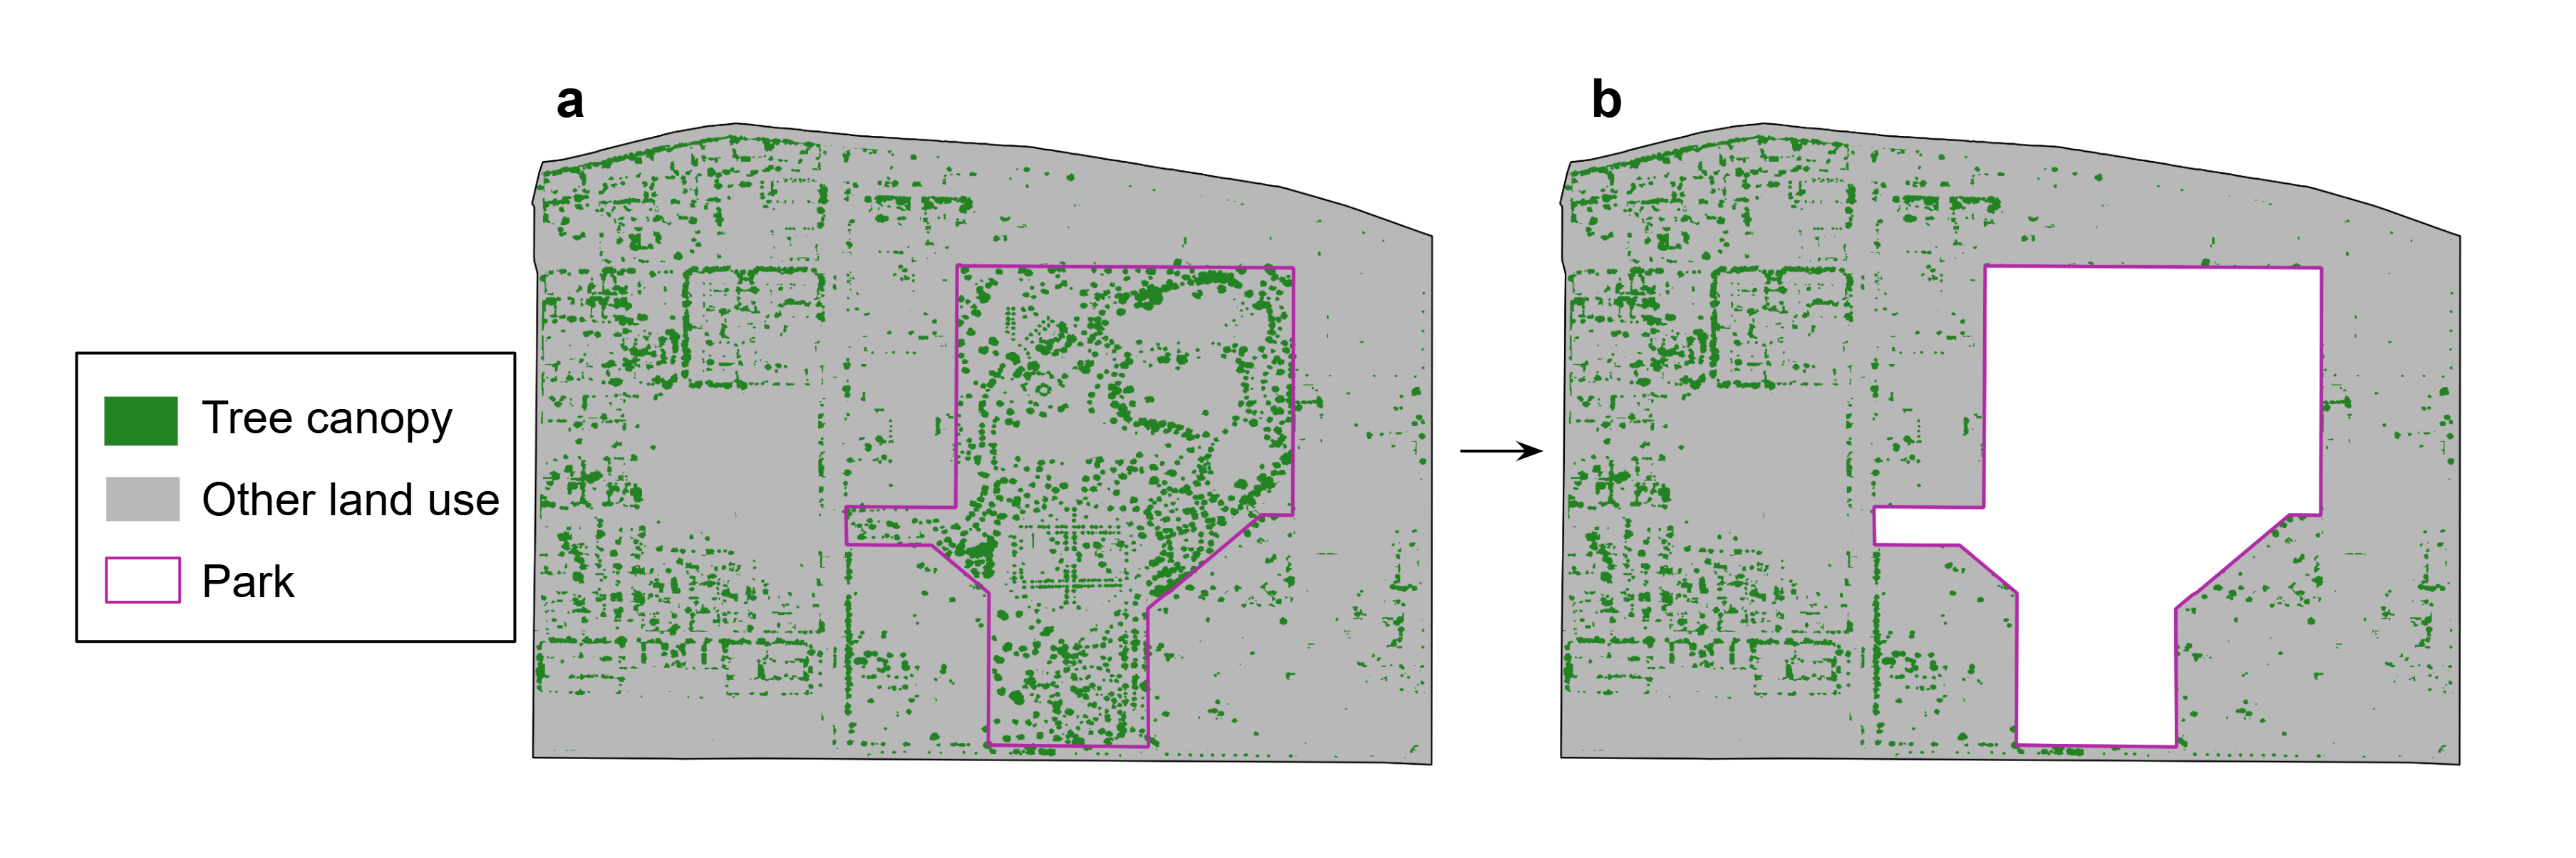
\includegraphics[keepaspectratio,alt={Map showing a block group with 11.7\% tree canopy cover. The tree canopy reduces to 8.2\% when a large park is clipped out of the block group.}]{images/fig-bg-tree-cover.png}}

}

\caption{\label{fig-tree-cover}The effect of public park tree canopy
cover on total tree canopy cover}

\end{figure}%

The Mann-Whitney \emph{U} test was performed to determine whether TTCC
within block groups is affected by the presence of public parks. The
median TTCC value of the 176 block groups with parks was compared to the
TTCC value of the 841block groups without parks, and the \emph{U}
statistic was calculated.

The Wilcoxon signed-rank test was performed on the block groups that
contain public parks to determine whether the parks contribute to the
total tree canopy cover within those block groups.

\subsection{Demographic factors}\label{sec-demographic}

Total population and race/ethnicity data at the block group level were
sourced from the 2024 American Community Survey (ACS) 5-year estimate
{[}18{]} using the tidycensus R package. These factors were used to
calculate the percentage of Black and Hispanic residents per block
group. Population estimates from the 2024 ACS 5-year estimate were also
downloaded for individual Census blocks to be used for calculating
population-weighted block group centroids.

The area deprivation index (ADI) at the block group level was acquired
from the University of Wisconsin School of Medicine Public Health
{[}19{]}. The ADI is a validated measure of socioeconomic status based
on 17 indicators of income, education, employment, and housing quality
{[}20{]}. The raw ADI score of a block group is compared against all
other block groups in the nation and ranked on a percentile scale from
1-100, where 1 indicates the lowest level of disadvantage and 100
indicates the highest disadvantage. Block groups containing
predominantly group housing (college dormitories or jails) do not have
ADI data available, so they were excluded from the analysis. The
resulting dataset contained 988 block groups used in the demographic
analysis. Figure~\ref{fig-bg-parks} shows the locations of block groups
with land cover and/or demographic data available and the types of
public parks within the block groups.

\protect\phantomsection\label{cell-fig-bg-parks}
\begin{figure}[H]

\centering{

\pandocbounded{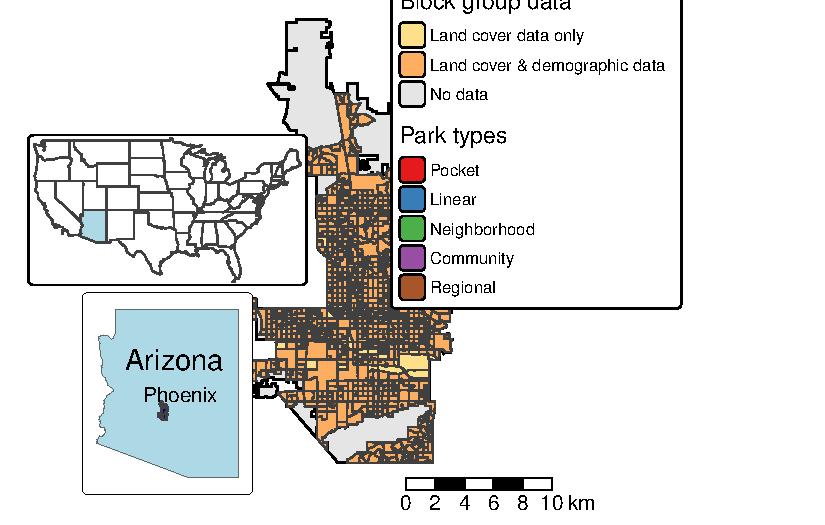
\includegraphics[keepaspectratio,alt={A map shows that most block groups in Phoenix have land cover and demographic data available; some only have land cover data; the five types of public parks are scattered throughout the city}]{index_files/figure-pdf/fig-bg-parks-1.pdf}}

}

\caption{\label{fig-bg-parks}Block groups and public parks in Phoenix,
Arizona}

\end{figure}%

Median household income is often used as a predictor variable in green
space access research {[} {[}7{]}, {[}10{]}{]}, but it was excluded from
this study due to its high correlation with ADI rank (\emph{r} = -0.70)
and the presence of 50 block groups with suppressed income estimates in
the ACS data.

\subsection{Spatial access to park tree canopy
cover}\label{sec-methods-spatial}

The Gaussian two-step floating catchment area (G2SFCA) method was used
to determine Phoenix residents' spatial access to tree canopy cover in
public parks. This method accounts for both the supply of public
amenities and demand on those amenities when calculating accessibility.
In previous studies of green space equity, park size and amenities have
often been used as the supply term (CITE). The population of areas
surrounding an amenity represents the demand on the amenity. More people
living near a park leads to greater competition for the park's
amenities, including tree canopy cover.

Park tree canopy area in hectares (PTCA) was used as the supply term in
this study and was calculated by multiplying the percent tree canopy
cover of a park by its total area (Table~\ref{tbl-parks}). Since PTCA
values are affected by both park size and percent tree canopy cover,
residents living near several small tree-dense parks may have access to
more tree canopy than residents near a single large park with scant tree
cover.

\begin{table}

\caption{\label{tbl-parks}Total park area and park tree canopy cover
area in Phoenix public parks}

\centering{

\fontsize{12.0pt}{14.0pt}\selectfont
\begin{tabular*}{\linewidth}{@{\extracolsep{\fill}}lrrrrr}
\toprule
  & Mean & SD & Median & Min & Max \\ 
\midrule\addlinespace[2.5pt]
Total park area (ha) & 8.30 & 12.51 & 4.46 & 0.08 & 115.25 \\ 
Park tree canopy area (ha) & 1.08 & 1.53 & 0.60 & 0.00 & 14.13 \\ 
\bottomrule
\end{tabular*}
\begin{minipage}{\linewidth}
\vspace{.05em}
\parbox{\linewidth}{\raggedright {\emph{N} = 177}}\\
\end{minipage}

}

\end{table}%

The original 2SFCA, developed by Luo and Wang (2003) {[}21{]}, considers
an amenity to be fully accessible if it lies within a given travel time
or distance from a residential area and fully inaccessible if it lies
outside this catchment area. However, the decision to visit an amenity
is not dichotomous; for example, a resident may choose to travel farther
to visit a park with more tree canopy even though there are other parks
nearby that provide less shade. The Gaussian 2SFCA method used in this
study improves on the original method by applying a continuous weighting
function to the travel distance, where nearby parks are given more
weight than those farther away within the same catchment area. Residents
who choose more distant parks will thus encounter greater travel
friction {[}22{]}.

The first step in the G2SFCA method is to compute the ratio of park tree
canopy area to the surrounding block group population at each park
location. The population-weighted centroid of block groups was used as
the population location (\(k\)) in calculating the distance between
block groups and parks. This point represents the mean location of
residents within the block group. Populations at each block group
location \(k\) are weighted using a Gaussian function. This ratio is
calculated as:

\begin{equation}\protect\phantomsection\label{eq-sd-ratio}{R_j = \frac{S_j}{\sum_{k \in {d_{kj} \leq d_0}} G(d_{kj}, d_0)P_k},}\end{equation}

where \(P_k\) is the population at block group \(k\) whose
population-weighted centroid lies within the catchment (i.e.,
\(d_{kj} \leq d_0\)) of a park at location \(j\); \(d_{kj}\) is the
travel distance between block group \(k\) and park \(j\); \(S_j\) is the
supply capability of park \(j\), i.e., the tree canopy area in hectares;
\(G\) is the friction-of-distance, calculated below:

\begin{equation}\protect\phantomsection\label{eq-gaussian}{G(d_{kj}, d_0) = 
\begin{cases}
\dfrac{e^{-(1/2) \times (d_{kj}/d_0)^2} - e^{-(1/2)}}{1 - e^{-(1/2)}}, & \text{if } d_{kj} \leq d_0 \\[10pt]
0, & \text{if } d_{kj} > d_0
\end{cases} .}\end{equation}

The second step in G2SFCA is to search all parks \(l\) within the
threshold distance \(d_0\) from block group \(i\), thus creating the
catchment for the population at \(i\). Each \(R\) is discounted using
the Gaussian function \(G\). The discounted \(R\) values within the
catchment area of \(i\) are summed to obtain the spatial accessibility
of park tree canopy area at block group \(i\) as follows:

\begin{equation}\protect\phantomsection\label{eq-access}{A_i = \sum_{l \in \ d_{il} \leq d_0} G (d_{il}, d_0)R_l,}\end{equation}

where \(l\) denotes all parks within the catchment of block group \(i\),
and all other notations are the same as in Equation~\ref{eq-sd-ratio}.
The park tree canopy accessibility score (\(A_i\)) represents the amount
of park tree canopy cover (in hectares) available to each resident in a
given block group. Raw accessibility scores are very small values and
thus were re-scaled by a factor of 1,000,000 for reporting purposes; the
re-scaled values are hereafter referred to as park tree access scores
(PTAS).

Public park access studies often use the park centroid as the
destination point. However, this can bias the results against large
parks since users may have to walk long distances from a park entrance
to the centroid. Parks may also have multiple points of entry that are
separated by significant distances {[}23{]}. This study used park
entrances, determined by visual examination using QGIS, as destination
locations for parks larger than 2 ha. For smaller parks, the centroid
was used since travel time would be minimally affected by the access
point location.

Travel distance (\(d_{kj}\)) from block group centroids (\(k\)) to park
entrances (\(j\)) was computed using the driving profile in the osrm R
package {[}24{]}. This method uses the Open Source Routing Machine to
identify the shortest driving path between any two points based on the
OpenStreetMap road network. A distance matrix of all block group
population-weighted centroids to all park entrances was created and then
limited to the distance from a block group to only the nearest entrance
within any given park.

Park catchment size (\(d_0\)) was determined by the service area radius
assigned to each park category by the City of Phoenix {[}25{]}. Pocket
and linear parks were assigned a threshold of 0.8 km (0.5 mi),
neighborhood parks 1.6 km (1 mi), community parks 4.8 km (3 mi), and
regional parks 8.0 km (5 mi). This aligns the park catchment values with
the park accessibility goals of the City of Phoenix.

The G2SFCA method is vulnerable to the ``edge effect'' problem wherein
phenomena contributing to the spatial patterns of an analysis unit may
lie outside of that unit {[}26{]}. In other words, accessibility scores
for block groups on the periphery of Phoenix may be negatively impacted
if block groups from surrounding cities are not included in the
analysis. This is because residents of these other cities can use
Phoenix parks, thus diluting the amount of tree cover available to
Phoenix residents. The edge effect was accounted for in the demand
portion of the method because the populations of 682 block groups from
surrounding cities that lie within a park catchment area were included
in the calculation of the supply/demand ratios (\(R_j\) and \(R_l\)).
The edge effect can also impact the supply of park tree canopy area
since Phoenix residents can access parks in other cities. However, this
is not relevant to the current study because the purpose was to measure
the access of residents only to those parks maintained by the City
Phoenix. Hence, public parks located in nearby cities were not included
in the analysis.

\subsection{Regression analysis of tree canopy cover
disparities}\label{sec-methods-regress}

Evaluating demographic disparities in block group-level tree canopy
cover began with ordinary least squares (OLS) regression models using
RTCC and PTAS as the predictor variables and percent Hispanic
population, percent Black population, and ADI national percentile rank
as the independent variables. An initial OLS model using the
untransformed PTAS score showed non-normal residuals (Shapiro-Wilk
\emph{W} = 0.843, \emph{p} \textless{} .001) with visible right skew in
a Q-Q plot. A square root transformation was applied to PTAS and the
model re-estimated; residual normality improved substantially (\emph{W}
= 0.955) but remained significantly non-normal (\emph{p} \textless{}
.001). Percent White population was excluded from the analyses due to
collinearity with the percent Hispanic population. Percent of the
population under 18 years old and over 64 years old were considered as
predictors, but both had an insignificant impact on the OLS results.

Demographic and environmental variables often exhibit spatial
autocorrelation, meaning the residuals in a given block group are likely
to be similar to their surrounding block groups. The presence of spatial
autocorrelation violates the assumption of independent residuals
necessary for OLS regression, necessitating the use of spatially aware
regression models. The global Moran's \emph{I} index was calculated to
measure the overall spatial autocorrelation of the residuals of both OLS
regression models using the following formula:

\begin{equation}\protect\phantomsection\label{eq-morans}{I = \frac{N}{S_0} \frac {\sum_{i=1}^N \sum_{j=1}^N w_{ij}(x_i-\bar x) (x_j-\bar x)} {\sum_{i=1}^N (x_i-\bar x)^2},}\end{equation}

where \(N\) is the number of block groups indexed by \(i\) and \(j\),
\(x\) is the variable of interest (i.e., OLS residuals), \(\bar{x}\) is
the mean of \(x\)\emph{,} \(w_{ij}\) is a spatial weights matrix that
represents the degree of spatial proximity between block groups \(i\)
and \(j\). The distance matrix was calculated based on the eight nearest
neighbors of each block group. This method allowed for all block groups
to be included in the computation, resulting in no isolated ``islands''
of block groups. A Monte Carlo simulation with 999 iterations was used,
and the \emph{p}-value was set at 0.01 to evaluate the significance of
the global Moran's \emph{I} index. The value of Moran's \emph{I} ranges
from -1 to 1; positive values indicate clustering, negative values
indicate dispersion, and 0 indicates a random distribution of residuals.

Since spatial autocorrelation was present in the residuals of the OLS
models for both dependent variables, spatial regression models were
warranted. Lagrange Multiplier (LM) tests were used to determine the
appropriate spatial regression specification for each outcome, following
the decision rule recommended by Anselin and Serge {[}27{]}: if the
robust LM error statistic is significant and the robust LM lag statistic
is not, a spatial error model is selected; if robust LM lag is
significant and robust LM error is not, a spatial lag model is selected.
LM tests indicated that a spatial error specification was appropriate
for both RTCC and PTAS (see Section~\ref{sec-results}).

In a spatial error model, spatial dependence is captured in the error
term rather than the outcome itself. This specification is appropriate
when neighboring block groups have similar residuals due to unmeasured
place-based factors that cluster spatially and affect tree canopy cover,
such as housing age or homeowners association planting guidelines. By
modeling this spatial structure as an error term, the spatial error
model isolates the independent effects of racial/ethnic composition and
socioeconomic disadvantage on tree canopy outcomes. The spatial error
model takes the following form:

\begin{equation}\protect\phantomsection\label{eq-sem}{y = X \beta + u,}\end{equation}

where \(y\) is the outcome (RTCC or PTAS), \(X\) represents the
predictor variables (percent Hispanic population, percent Black
population, and ADI rank), \(\beta\) represents the coefficients, and
\(u\) is an error term modeled as:

\begin{equation}\protect\phantomsection\label{eq-error}{u = \lambda Wu + \epsilon,}\end{equation}

where \(\lambda\) is the spatial error coefficient, \(Wu\) is the
weighted average of neighboring errors based on a spatial weights matrix
of the eight nearest neighbors, and \(\epsilon\) is a random independent
error term.

\subsection{Compensatory tree canopy access (need better
title)}\label{sec-methods-multinom}

After separately identifying spatial patterns in residential tree canopy
cover and public park tree access scores, block groups were classified
as either high RTCC or low RTCC. Those with a RTCC of 15\% or higher
were classified into the high RTCC category and the rest were considered
low RTCC. This threshold is based on the recommendation of the
non-profit organization American Forests that desert cities should
maintain a 15\% tree canopy cover to achieve tree equity {[}28{]}. In
the absence of a clear policy guideline for park tree access score,
block groups with a PTAS below the median were categorized as low PTAS,
and those at or above the median were categorized as high PTAS. The two
factors were then combined to create four tree canopy access categories:
a) high RTCC/high PTAC (HH), b) high RTCC/low PTAS (HL), c) low
RTCC/high PTAS (LH), or d) low RTCC/low PTAS (LL).

Multinomial logistic regression was used to examine whether the percent
Hispanic, percent Black, or ADI rank predicted a block group's
membership in each tree canopy access category relative to the high
RTCC/high PTAS condition (HH). Given that spatial autocorrelation was
detected in the residuals of both the RTCC and PTAS regression
residuals, it was expected that the residuals of the tree access
category logistic regression model might exhibit similar spatial
dependence. However, global Moran's \emph{I} cannot be calculated
directly on the residuals of a multinomial logistic model, since the
outcome comprises four unordered categories rather than a single
continuous or binary residual vector. To address this, each tree canopy
access category (HH, HL, LH, LL) was recast as a binary outcome
(one-vs-rest) and modeled separately via logistic regression on the same
three demographic predictors. Global Moran's \emph{I} was then
calculated on the residuals of each binary model to test for spatial
autocorrelation.

Significant spatial autocorrelation was detected on the residuals of all
four binary regression models (see Section~\ref{sec-results}), so the
Moran eigenvector spatial filtering approach was used to incorporate
spatial predictors into the models {[}29{]}. This approach decomposes a
spatial weights matrix into orthogonal eigenvectors, each representing a
distinct spatial pattern at a different scale. These eigenvectors are
incorporated into regression model as additional predictors, thereby
absorbing the spatial signal that would otherwise be part of the model's
error term. Eigenvector selection was implemented using the spatialreg R
package {[}30{]}, using the eight nearest-neighbors matrix used
previously. Each eigenvector was tested iteratively, and those that
significantly reduced Moran's \emph{I} (α = 0.08) were retained. The
selected eigenvectors were added as additional covariates to each binary
logistic model, and global Moran's \emph{I} was recalculated on the
resulting residuals to assess the degree to which spatial
autocorrelation had been reduced.

\section{Results}\label{sec-results}

\subsection{Impact of public parks on tree canopy
cover}\label{sec-res-impact}

Percent total tree canopy cover (TTCC) is the amount of tree canopy
cover in a block group including the tree cover provided by public
parks. Across the entire city, the 176 block groups that contain parks
have a median TTCC of 10.95, while the 841 block groups without parks
have a median TTCC of 11.17. This difference is non-significant
(Mann-Whitney \emph{U} = 78897, \emph{p} = 0.168), suggesting that parks
are evenly distributed across the canopy spectrum rather than
concentrated in already-green neighborhoods.

Percent residential tree canopy cover (RTCC) is the tree cover in a
block group excluding the tree cover provided by public parks. TTCC and
RTCC were compared in the 176 block groups that contain parks to
determine whether the parks significantly contribute to block
group-level tree canopy cover in Phoenix. The median TTCC was 10.20\%,
while RTCC was higher at 10.95\% . This difference was statistically
significant (Wilcoxon signed-rank test, \emph{V} = 11271, \emph{p}
\textless{} 0.001), confirming that parks meaningfully contribute to
tree canopy cover when they are present in a neighborhood.
Table~\ref{tbl-ttcc-rtcc} (mention how parks sometimes reduce canopy
cover)

\begin{table}

\caption{\label{tbl-ttcc-rtcc}Total tree canopy cover and residential
tree canopy cover in block groups that contain parks}

\centering{

\fontsize{12.0pt}{14.0pt}\selectfont
\begin{tabular*}{\linewidth}{@{\extracolsep{\fill}}lrrrrr}
\toprule
 & Mean & SD & Median & Min & Max \\ 
\midrule\addlinespace[2.5pt]
Total tree canopy cover (\%) & 11.47 & 4.19 & 10.95 & 3.65 & 26.28 \\ 
Residential tree canopy cover (\%) & 11.25 & 4.36 & 10.20 & 3.49 & 27.50 \\ 
Difference between TTCC and RTCC & 0.23 & 0.74 & 0.12 & -2.59 & 3.94 \\ 
\bottomrule
\end{tabular*}
\begin{minipage}{\linewidth}
\vspace{.05em}
\parbox{\linewidth}{\raggedright {\emph{N} = 176 block groups}}\\
\end{minipage}

}

\end{table}%

\subsection{Regression analysis}\label{sec-res-regress}

Table~\ref{tbl-desc-stats} presents descriptive statistics for the block
group characteristics and outcome variables (RTCC and PTAS) used in the
regression analyses. Block group population is included for reference,
but it was not used as a predictor variable. Maps of RTCC and PTAS are
shown in Figure~\ref{fig-ptcc-ptas-map}, and maps of the three predictor
variables (percent Hispanic population, percent Black population, and
ADI rank) are depicted in Figure~\ref{fig-bg-demographics}.

\begin{table}

\caption{\label{tbl-desc-stats}Descriptive statistics of the dataset}

\centering{

\fontsize{12.0pt}{14.0pt}\selectfont
\begin{tabular*}{\linewidth}{@{\extracolsep{\fill}}lrrrrr}
\toprule
 & Mean & SD & Median & Min & Max \\ 
\midrule\addlinespace[2.5pt]
\multicolumn{6}{l}{\emph{Block group characteristics}} \\[2.5pt] 
\midrule\addlinespace[2.5pt]
Total population & 1,597 & 710 & 1,499 & 102 & 6,221 \\ 
Hispanic population (\%) & 39.7 & 28.7 & 33.9 & 0.0 & 99.3 \\ 
Black population (\%) & 6.8 & 9.5 & 3.0 & 0.0 & 59.1 \\ 
ADI rank & 40 & 19 & 40 & 1 & 100 \\ 
\midrule\addlinespace[2.5pt]
\multicolumn{6}{l}{\emph{Outcome variables}} \\[2.5pt] 
\midrule\addlinespace[2.5pt]
Residential tree canopy cover (\%) & 11.9 & 4.3 & 11.1 & 2.6 & 28.2 \\ 
Park tree canopy access score & 105.6775 & 58.48181 & 97.3453 & 1.445721 & 567.9618 \\ 
\bottomrule
\end{tabular*}
\begin{minipage}{\linewidth}
\vspace{.05em}
\parbox{\linewidth}{\raggedright {\emph{N} = 988 block groups}}\\
\end{minipage}

}

\end{table}%

\protect\phantomsection\label{cell-fig-ptcc-ptas-map}
\begin{figure}[H]

\centering{

\pandocbounded{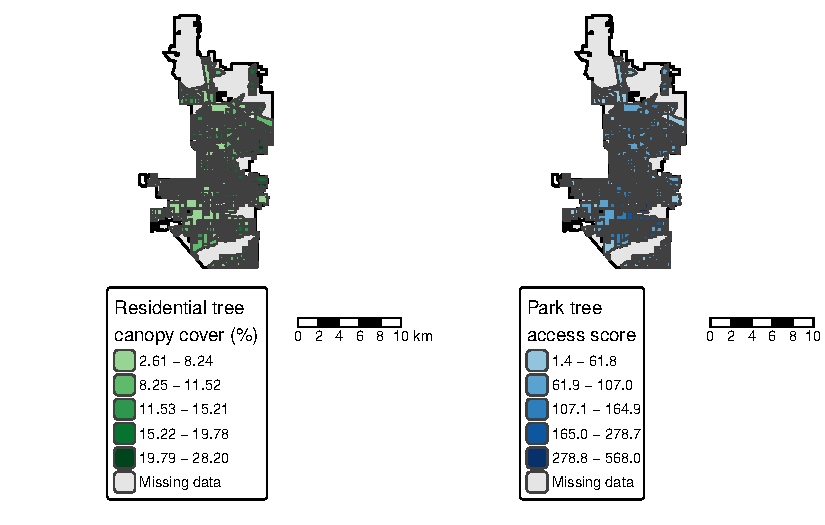
\includegraphics[keepaspectratio,alt={Residential tree canopy cover is highest in the central and northeastern parts of Phoenix. Park tree access score is highest in the central part.}]{index_files/figure-pdf/fig-ptcc-ptas-map-1.pdf}}

}

\caption{\label{fig-ptcc-ptas-map}Residential tree canopy cover (\%) and
park tree access score of Phoenix block groups}

\end{figure}%

\protect\phantomsection\label{cell-fig-bg-demographics}
\begin{figure}[H]

\centering{

\pandocbounded{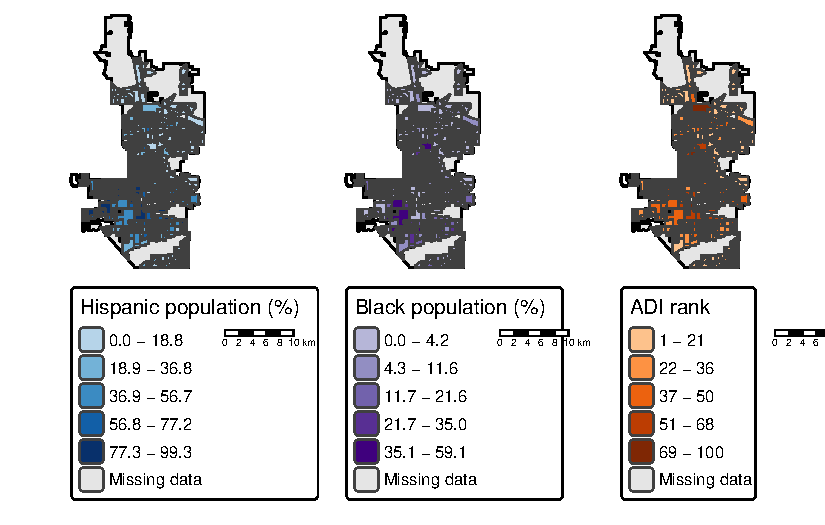
\includegraphics[keepaspectratio,alt={Hispanic population is highest in the southwestern part of Phoenix; Black population is highest in the southern part with a small pocket in the north; ADI rank is highest in the western part with a high cluster in the north}]{index_files/figure-pdf/fig-bg-demographics-1.pdf}}

}

\caption{\label{fig-bg-demographics}Maps of Hispanic population (\%),
Black population (\%), and ADI national percentile rank in Phoenix block
groups}

\end{figure}%

Based on the OLS model, percent Hispanic population, percent Black
population, and ADI rank were all negatively associated with RTCC
(\emph{p} \textless{} 0.001; see Table~\ref{tbl-regress}). For every 1\%
increase in the Hispanic population, residential tree canopy cover
within a block group is expected to decrease by 3.5\%; a 1\% increase in
the population of Black residents is associated with a 7.3\% decrease in
RTCC; and a 1-point increase in the ADI rank is associated with an 8.5\%
decrease in RTCC.

The percentage of Hispanic residents in a block group is not
significantly associated with the square root of PTAS, but there was a
significant positive association between the square root of PTAS and
both Black resident percentage (\emph{p} \textless{} 0.05) and ADI rank
(\emph{p} \textless{} 0.001; see Table~\ref{tbl-regress}).

These findings suggest that while neighborhoods with a higher Black
population and lower socioeconomic status have lower tree canopy cover
provided by trees on private property, street trees, and trees in
private parks, the public parks near these neighborhoods provide greater
access to tree canopy cover than those near neighborhoods with lower
Black populations and higher socioeconomic status.

Global Moran's \emph{I} was significant (\emph{p} \textless{} 0.001) for
both the RTCC and PTAS residuals from the OLS models. The RTCC index was
0.221, indicating moderate spatial clustering of residential tree canopy
values, and the PTAS index was 0.418, indicating strong spatial
clustering of park tree access scores.

Spatial error model results are presented in Table~\ref{tbl-regress}
along with OLS estimates for comparison. Similar to the OLS model, all
three predictor variables are negatively correlated with RTCC,
indicating that block groups with larger Hispanic populations, larger
Black populations, or higher ADI rank are more likely to have lower
residential tree canopy cover.

The spatial error model for the square-root transformed PTAS also
indicates that there is no correlation between park tree access and
Hispanic population percent. The coefficient of 0.019 for the Black
population percent (significant only at the \emph{p} \textless{} 0.1
level) suggests that there may be a slight increase in park tree access
as the Black population increases. The significant positive relationship
between PTAS and ADI rank indicates that the park tree access score
increases as socioeconomic status decreases.

The lambda (\(\lambda\)) term indicates how neighboring observations
influence one another's errors. The positive \(\lambda\) in both spatial
error models indicates that unmeasured error in one block group
significantly impacts the errors in adjoining block groups for both RTCC
and PTAS.

\begin{table}

\caption{\label{tbl-regress}Results of OLS and spatial error regression
models for RTCC and PTAS}

\centering{

\fontsize{12.0pt}{14.0pt}\selectfont
\begin{tabular*}{\linewidth}{@{\extracolsep{\fill}}lcccc}
\toprule
 & \multicolumn{2}{c}{{RTCC models}} & \multicolumn{2}{c}{{√PTAS models}} \\ 
\cmidrule(lr){2-3} \cmidrule(lr){4-5}
  & OLS & Spatial error & OLS  & Spatial error  \\ 
\midrule\addlinespace[2.5pt]
(Intercept) & 20.703*** & 17.199*** & 5.227*** & 8.541*** \\ 
Hispanic population (\%) & -0.037*** & -0.040*** & -0.007† & 0.000 \\ 
Black population (\%) & -0.064*** & -0.069*** & 0.011 & 0.019* \\ 
adi & -0.065*** &  & 0.046*** &  \\ 
ADI rank &  & -0.080*** &  & 0.027*** \\ 
lambda &  & 0.462*** &  & 0.731*** \\ 
\bottomrule
\end{tabular*}
\begin{minipage}{\linewidth}
\vspace{.05em}
\parbox{\linewidth}{\raggedright {* \emph{p} \textless{} 0.05, ** \emph{p} \textless{} 0.01, *** \emph{p} \textless{} 0.001}}\\
\parbox{\linewidth}{\raggedright {\emph{N} = 988}}\\
\end{minipage}

}

\end{table}%

\subsection{Demographic inequities in tree canopy
access}\label{sec-res-demographic}

Block groups were organized into one of four tree canopy access
categories based on their RTCC and PTAS values
(Table~\ref{tbl-canopy-access}). The spatial distribution of each
category is illustrated in Figure~\ref{fig-canopy-access-map}. The least
common category is HH, or neighborhoods with both abundant residential
tree canopy and higher than average access to park tree canopy. These
block groups are mostly confined to isolated pockets in the northeastern
part of Phoenix. Block groups in the HL category have lower than average
access to park trees, but the residential tree canopy is abundant. The
most common category is LH, representing block groups with low
residential tree canopy but high access to park canopy cover. These are
low-canopy neighborhoods where public parks provide a tree canopy refuge
to the residents. They are located mostly in the center and northern
portions of the city where most of the public parks are situated. The
remaining block groups belong to the LL category, or ``tree canopy
deserts,'' lacking both residential tree canopy cover and access to
public park tree canopy. They tend to be found on the periphery of the
city.

\begin{table}

\caption{\label{tbl-canopy-access}Tree canopy access categories}

\centering{

\fontsize{12.0pt}{14.0pt}\selectfont
\begin{tabular*}{\linewidth}{@{\extracolsep{\fill}}lllr}
\toprule
Category & Rule & Description & \emph{n} Block groups (\%) \\ 
\midrule\addlinespace[2.5pt]
HH & High RTCC + High PTAS & Abundant residential and park tree canopy & 89 (9.0) \\ 
HL & High RTCC + Low PTAS & Self-sufficient residential tree canopy & 122 (12.3) \\ 
LH & Low RTCC + High PTAS & Park tree canopy refuge & 404 (40.9) \\ 
LL & Low RTCC + Low PTAS & Tree canopy desert & 373 (37.8) \\ 
\bottomrule
\end{tabular*}
\begin{minipage}{\linewidth}
\vspace{.05em}
\parbox{\linewidth}{\raggedright {\emph{N} = 988 total block groups}}\\
\end{minipage}

}

\end{table}%

\protect\phantomsection\label{cell-fig-canopy-access-map}
\begin{figure}[H]

\centering{

\pandocbounded{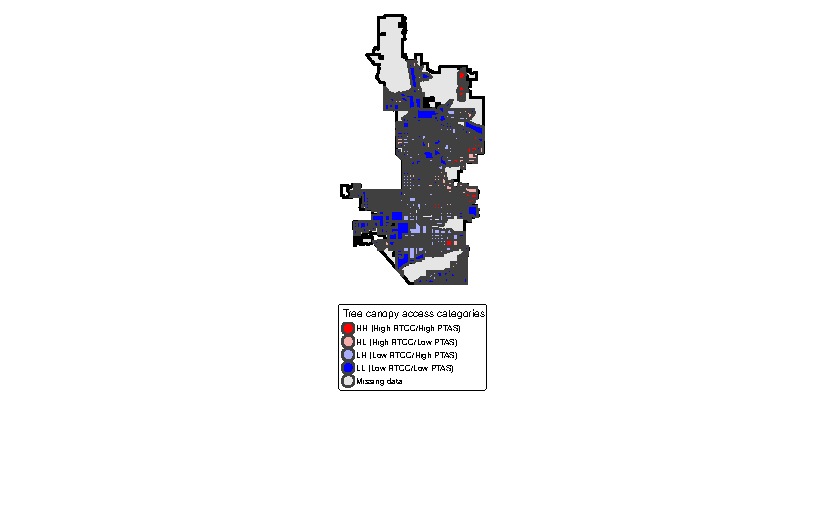
\includegraphics[keepaspectratio,alt={HH block groups are mostly in the northeast of Phoenix; HL block groups are in the eastern part; LH are mostly in the central part; LL are mostly on the edges of the city}]{index_files/figure-pdf/fig-canopy-access-map-1.pdf}}

}

\caption{\label{fig-canopy-access-map}Tree canopy access categories of
Phoenix block groups}

\end{figure}%

The multinomial logistic regression model estimates the odds that a
particular demographic factor (Hispanic population, Black population, or
ADI rank) predicts whether a block group belongs to either the HL, LH,
or LL tree access category rather than the baseline HH category. The
results show that block groups are equally likely to be in the HL
category compared to the HH category, regardless of the demographic
makeup of the block group. In other words, neighborhoods with high
residential tree canopy cover and high park tree canopy access are not
demographically distinct from those with high residential canopy and low
park tree access (Table~\ref{tbl-multinom}).

\begin{table}

\caption{\label{tbl-multinom}Multinomial logistic regression odds ratios
for canopy access categories}

\centering{

\fontsize{12.0pt}{14.0pt}\selectfont
\begin{tabular*}{\linewidth}{@{\extracolsep{\fill}}l>{\raggedleft\arraybackslash}p{\dimexpr 0.15\linewidth -2\tabcolsep-1.5\arrayrulewidth}>{\raggedleft\arraybackslash}p{\dimexpr 0.15\linewidth -2\tabcolsep-1.5\arrayrulewidth}>{\raggedleft\arraybackslash}p{\dimexpr 0.15\linewidth -2\tabcolsep-1.5\arrayrulewidth}>{\raggedleft\arraybackslash}p{\dimexpr 0.15\linewidth -2\tabcolsep-1.5\arrayrulewidth}>{\raggedright\arraybackslash}p{\dimexpr 0.15\linewidth -2\tabcolsep-1.5\arrayrulewidth}>{\raggedleft\arraybackslash}p{\dimexpr 0.15\linewidth -2\tabcolsep-1.5\arrayrulewidth}}
\toprule
 & \multicolumn{2}{>{\centering\arraybackslash}m{\dimexpr 0.30\linewidth -2\tabcolsep-1.5\arrayrulewidth}}{\parbox{\linewidth}{\centering {HL}}} & \multicolumn{2}{>{\centering\arraybackslash}m{\dimexpr 0.30\linewidth -2\tabcolsep-1.5\arrayrulewidth}}{\parbox{\linewidth}{\centering {LH}}} & \multicolumn{2}{>{\centering\arraybackslash}m{\dimexpr 0.30\linewidth -2\tabcolsep-1.5\arrayrulewidth}}{\parbox{\linewidth}{\centering {LL}}} \\ 
\cmidrule(lr){2-3} \cmidrule(lr){4-5} \cmidrule(lr){6-7}
Predictor & OR\textsuperscript{\textit{1}} & 95\% CI & OR & 95\% CI & OR & 95\% CI \\ 
\midrule\addlinespace[2.5pt]
Hispanic population (\%) & 1.00 & 0.98, 1.02 & 1.02* & 1.00, 1.03 & 1.01 & 1.00, 1.03 \\ 
Black population (\%) & 0.99 & 0.94, 1.05 & 1.05* & 1.01, 1.10 & 1.04† & 1.00, 1.08 \\ 
ADI rank & 0.99 & 0.96, 1.01 & 1.08** & 1.05, 1.10 & 1.06** & 1.03, 1.08 \\ 
\bottomrule
\end{tabular*}
\begin{minipage}{\linewidth}
\vspace{.05em}
\parbox{\linewidth}{\raggedright {Reference category: HH (High RTCC/High PTAS)}}\\
\parbox{\linewidth}{\raggedright {† \emph{p} \textless{} 0.1, * \emph{p} \textless{} 0.05, ** \emph{p} \textless{} 0.01}}\\
\parbox{\linewidth}{\raggedright {\emph{N} = 988: HH = 89 (9.0\%), HL = 122 (12.3\%), LH = 404 (40.9\%), LL = 373 (37.8\%)}}\\
\parbox{\linewidth}{\raggedright {\textsuperscript{\textit{1}}OR: Odds ratio; CI: Confidence interval}}\\
\end{minipage}

}

\end{table}%

All three demographic factors were significantly associated with
membership in the LH category (\emph{p}\textless0.05). For every 1\%
increase in the Hispanic population, there is a 2\% increase in the odds
that a block group belongs to the LH category vs.~the HH category. A 1\%
increase in Black population is associated with a 5\% increase in the
odds of belonging to the LH category. A one-point increase in ADI
national percentile rank is associated with an 8\% increase in the odds
of being in the LH category.

For the LL tree access category, only ADI rank is significant
(\emph{p}\textless0.001). For every one-point increase in ADI rank,
there is a 6\% increase in the odds that a block group belongs to this
category compared to the HH category.

Higher ADI rank was associated with greater odds of belonging to both
low RTCC categories, LH and LL, relative to HH. This supports the
previous finding that low socioeconomic status is linked to reduced
residential tree canopy cover in Phoenix. But there is no clear
relationship between the socioeconomic level of a block group and its
likelihood of having greater access to public park tree canopy cover.

The higher odds of a block group with a larger Black or Hispanic
population belonging to the LH category suggests that these
neighborhoods are more likely to have parks that act as tree canopy
refuges, providing higher park tree canopy access despite having low
residential tree canopy cover.

Because spatial autocorrelation was detected in the one-vs-rest binary
logistic models underlying the four-category canopy access typology
(Moran's \emph{I}: HH = 0.140, HL = 0.144, LH = 0.267, LL = 0.232; all
\emph{p} \textless{} 0.001), Moran eigenvector spatial filtering was
applied to the models. Selected eigenvectors (HH: 9, HL: 14, LH: 30, LL:
23) were added as covariates to each binary model, substantially
reducing spatial autocorrelation across all four categories. Moran's
\emph{I} was reduced by 76-85\% in each model (HH = 0.033, HL = 0.030,
LH = 0.040, LL = 0.034), though modest statistically significant spatial
clustering remained in each case (\emph{p} \textless{} 0.05). This
result is consistent with spatial structure operating at a scale broader
than the local nearest-neighbor weighting could capture.

Table~\ref{tbl-bin-regress} reports the β coefficients for each tree
canopy access binary logistic models before and after spatial filtering.
Both the HH and HL categories were negatively associated with ADI
national percentile rank, while the LH and LL categories were positively
associated with ADI rank. These associations were significant both
before and after spatial filtering, indicating that the relationship
between ADI and canopy access category is robust to the presence of
spatial autocorrelation in the model residuals. Significance levels for
most other predictor β terms also remained stable after filtering, with
two exceptions: for the HH category, the negative associations with
Hispanic population and Black population moved from marginal
significance (\emph{p} \textless{} 0.1) to significance at \emph{p}
\textless{} 0.05; and for HL, the negative association with Hispanic
population shifted from non-significant to significant at \emph{p}
\textless{} 0.05, while the association with Black population
strengthened from \emph{p} \textless{} 0.05 to \emph{p} \textless{}
0.01.

\begin{table}

\caption{\label{tbl-bin-regress}Binary logistic regression results for
canopy access categories before and after spatial filtering}

\centering{

\fontsize{12.0pt}{14.0pt}\selectfont
\begin{tabular*}{\linewidth}{@{\extracolsep{\fill}}l|lr}
\toprule
Term & β (unfiltered) & β (filtered) \\ 
\midrule\addlinespace[2.5pt]
\multicolumn{3}{l}{{\itshape HH}} \\[2.5pt] 
\midrule\addlinespace[2.5pt]
Intercept & -0.303 & -0.778** \\ 
Hispanic population (\%) & -0.013† & -0.018* \\ 
Black population (\%) & -0.035† & -0.041* \\ 
ADI rank & -0.044*** & -0.039*** \\ 
\midrule\addlinespace[2.5pt]
\multicolumn{3}{l}{{\itshape HL}} \\[2.5pt] 
\midrule\addlinespace[2.5pt]
Intercept & 0.577** & 0.628* \\ 
Hispanic population (\%) & -0.01 & -0.021** \\ 
Black population (\%) & -0.043* & -0.066** \\ 
ADI rank & -0.065*** & -0.068*** \\ 
\midrule\addlinespace[2.5pt]
\multicolumn{3}{l}{{\itshape LH}} \\[2.5pt] 
\midrule\addlinespace[2.5pt]
Intercept & -2.13*** & -2.533*** \\ 
Hispanic population (\%) & 0.007* & 0.006 \\ 
Black population (\%) & 0.019** & 0.025** \\ 
ADI rank & 0.032*** & 0.038*** \\ 
\midrule\addlinespace[2.5pt]
\multicolumn{3}{l}{{\itshape LL}} \\[2.5pt] 
\midrule\addlinespace[2.5pt]
Intercept & -0.76*** & -1.151*** \\ 
Hispanic population (\%) & 0.001 & 0.005 \\ 
Black population (\%) & 0.005 & 0.001 \\ 
ADI rank & 0.004 & 0.008 \\ 
\bottomrule
\end{tabular*}
\begin{minipage}{\linewidth}
\vspace{.05em}
\parbox{\linewidth}{\raggedright {† \emph{p} \textless{} 0.1, * \emph{p} \textless{} 0.05, ** \emph{p} \textless{} 0.01, *** \emph{p} \textless{} 0.001}}\\
\end{minipage}

}

\end{table}%

\section{Discussion}\label{sec-discussion}

This study examined the ability of Phoenix residents to access both
residential tree canopy cover and public park tree canopy cover.

\subsection{Public park contribution to tree canopy
cover}\label{public-park-contribution-to-tree-canopy-cover}

Public parks contribute to the total tree canopy cover found within
Phoenix neighborhoods. Although the average increase in tree cover is
small, it is statistically significant. On average, Phoenix
neighborhoods that contain parks have higher tree canopy cover than they
would have if the parks were not present.

\subsection{Inequitable distribution of tree canopy
cover}\label{inequitable-distribution-of-tree-canopy-cover}

This study confirms that tree canopy cover is inequitably distributed
across Phoenix. Previous studies have shown that total tree canopy cover
is highest in block groups with lower racial and ethnic minorities and
higher socioeconomic status. This study adds to these findings that this
pattern also applies to residential tree canopy cover, excluding the
tree canopy provided by public parks.

This is the first study to analyze access to public park tree canopy
cover in Phoenix. It is also the first study to use the Gaussian
two-step floating catchment area (G2SFCA) method to analyze access to
tree canopy cover in parks. This method is superior to traditional
measures of park access that only consider presence/absence of parks and
use a binary distance metric to determine access. G2SFCA accounts for
both tree canopy area and population-based demand on the tree canopy
while also applying distance-based weighting to the calculation of
distance from block groups to parks. The use of actual park entrances
for determining distance-to-park is also an improvement over centroid-
or perimeter-based methods that may over- or under-estimate the true
distances from residential areas to the parks. Zhang et al.~(2023) found
that the use of centroids in a park access study underestimated the
disparities in accessibility compared to the use of park entrances
{[}8{]}.

G2SFCA could be applied to other cities to determine whether access to
public tree cover is equitably distributed.

Park tree access score is better than amount of tree canopy area
available to each block group because it takes population demand into
account. Other studies focus on access to parks but don't consider park
tree cover as an amenity. Some studies

\subsection{Limitations and future
research}\label{limitations-and-future-research}

\section*{References}\label{references}
\addcontentsline{toc}{section}{References}

\protect\phantomsection\label{refs}
\begin{CSLReferences}{0}{1}
\bibitem[\citeproctext]{ref-wang2024}
\CSLLeftMargin{1. }%
\CSLRightInline{Wang Z, Fan C, Que X, Liao FH, Ma X, Wang H (2024)
Multi-scale analysis of urban forests and socioeconomic patterns in a
desert city, phoenix, arizona. Scientific Reports 14:23864.
https://doi.org/\href{https://doi.org/10.1038/s41598-024-74208-8}{10.1038/s41598-024-74208-8}}

\bibitem[\citeproctext]{ref-lara-valencia2018}
\CSLLeftMargin{2. }%
\CSLRightInline{Lara-Valencia F, Garcia-Perez H (2018) Disparities in
the provision of public parks in neighbourhoods with varied latino
composition in the phoenix metropolitan area. Local Environment
23:1107--1120.
https://doi.org/\href{https://doi.org/10.1080/13549839.2018.1528443}{10.1080/13549839.2018.1528443}}

\bibitem[\citeproctext]{ref-ibes2015}
\CSLLeftMargin{3. }%
\CSLRightInline{Ibes DC (2015) A multi-dimensional classification and
equity analysis of an urban park system: A novel methodology and case
study application. Landscape and Urban Planning 137:122--137.
https://doi.org/\href{https://doi.org/10.1016/j.landurbplan.2014.12.014}{10.1016/j.landurbplan.2014.12.014}}

\bibitem[\citeproctext]{ref-corley2024}
\CSLLeftMargin{4. }%
\CSLRightInline{Corley EA (2024) Environmental justice and phoenix,
arizona neighborhood parks. Environmental Justice 17:256--266.
https://doi.org/\href{https://doi.org/10.1089/env.2022.0054}{10.1089/env.2022.0054}}

\bibitem[\citeproctext]{ref-kim2023}
\CSLLeftMargin{5. }%
\CSLRightInline{Kim Y, Corley EA, Won Y, Kim J (2023) Green space access
and visitation disparities in the phoenix metropolitan area. Landscape
and Urban Planning 237:104805.
https://doi.org/\href{https://doi.org/10.1016/j.landurbplan.2023.104805}{10.1016/j.landurbplan.2023.104805}}

\bibitem[\citeproctext]{ref-kim_green_2023}
\CSLLeftMargin{6. }%
\CSLRightInline{Kim Y, Corley EA, Won Y, Kim J (2023) Green space access
and visitation disparities in the phoenix metropolitan area. Landscape
and Urban Planning 237:104805.
https://doi.org/\href{https://doi.org/10.1016/j.landurbplan.2023.104805}{10.1016/j.landurbplan.2023.104805}}

\bibitem[\citeproctext]{ref-lara-valencia_disparities_2018}
\CSLLeftMargin{7. }%
\CSLRightInline{Lara-Valencia F, Garcia-Perez H (2018) Disparities in
the provision of public parks in neighbourhoods with varied {Latino}
composition in the {Phoenix} {Metropolitan} {Area}. Local Environment
23:1107--1120.
https://doi.org/\href{https://doi.org/10.1080/13549839.2018.1528443}{10.1080/13549839.2018.1528443}}

\bibitem[\citeproctext]{ref-zhang_assessing_2023}
\CSLLeftMargin{8. }%
\CSLRightInline{Zhang D, Ma S, Fan J, Xie D, Jiang H, Wang G (2023)
Assessing spatial equity in urban park accessibility: An improve
two-step catchment area method from the perspective of 15-mintue city
concept. Sustainable Cities and Society 98:104824.
https://doi.org/\href{https://doi.org/10.1016/j.scs.2023.104824}{10.1016/j.scs.2023.104824}}

\bibitem[\citeproctext]{ref-kim2024}
\CSLLeftMargin{9. }%
\CSLRightInline{Kim K, Horner MW (2024) Assessing the effects of
centroid assignment methods on measuring spatial accessibility.
Transactions in GIS 28:2025--2043.
https://doi.org/\href{https://doi.org/10.1111/tgis.13228}{10.1111/tgis.13228}}

\bibitem[\citeproctext]{ref-zhou2013}
\CSLLeftMargin{10. }%
\CSLRightInline{Zhou X, Kim J (2013) Social disparities in tree canopy
and park accessibility: A case study of six cities in illinois using GIS
and remote sensing. Urban Forestry \& Urban Greening 12:88--97.
https://doi.org/\href{https://doi.org/10.1016/j.ufug.2012.11.004}{10.1016/j.ufug.2012.11.004}}

\bibitem[\citeproctext]{ref-quickfa}
\CSLLeftMargin{11. }%
\CSLRightInline{\href{https://www.census.gov/quickfacts/fact/table/phoenixcityarizona/PST045224}{Quick
facts: Phoenix city, arizona}}

\bibitem[\citeproctext]{ref-tidycensus}
\CSLLeftMargin{12. }%
\CSLRightInline{Walker K, Herman M (2026) Tidycensus: Load US census
boundary and attribute data as 'tidyverse' and 'sf'-ready data frames.
\url{https://doi.org/10.32614/CRAN.package.tidycensus}}

\bibitem[\citeproctext]{ref-openstre}
\CSLLeftMargin{13. }%
\CSLRightInline{\href{https://www.openstreetmap.org}{OpenStreetMap}}

\bibitem[\citeproctext]{ref-cityofphoenixb}
\CSLLeftMargin{14. }%
\CSLRightInline{City of Phoenix
\href{https://web-prod.phoenix.gov/content/dam/phoenix/pddsite/documents/planning-zoning-general-plan/parks-rec-facility-standards.pdf}{Parks
and recreation facility standards}}

\bibitem[\citeproctext]{ref-gallego2024}
\CSLLeftMargin{15. }%
\CSLRightInline{Gallego K, Stark D, O'Brien A, Waring J, Pastor L,
Guardado B, Robinson K, Galindo-Elvira C, Washington KH, Dalton K,
Barnwell A, Bustamente D, Moya A, Porter S, Viera E, Zuercher E, Cuilty
J, Fallon W, Furniss J (2024)
\href{https://www.phoenix.gov/content/dam/phoenix/parkssite/mediaassets/2024\%20Parks\%20Annual\%20Report\%20(1).pdf}{Parks
annual report}}

\bibitem[\citeproctext]{ref-cityofphoenixparksandrecreationdepartment}
\CSLLeftMargin{16. }%
\CSLRightInline{Phoenix Parks C of, Recreation Department Phoenix park
classifications}

\bibitem[\citeproctext]{ref-maricopa2021}
\CSLLeftMargin{17. }%
\CSLRightInline{(2021) Maricopa county AZ 1ft resolution land cover}

\bibitem[\citeproctext]{ref-uscensusbureau}
\CSLLeftMargin{18. }%
\CSLRightInline{US Census Bureau
\href{https://www.census.gov/programs-surveys/acs/}{American community
survey (ACS)}}

\bibitem[\citeproctext]{ref-universityofwisconsinschoolofmedicinepublichealth2023}
\CSLLeftMargin{19. }%
\CSLRightInline{University of Wisconsin School of Medicine Public Health
(2023) \href{https://www.neighborhoodatlas.medicine.wisc.edu/}{Area
deprivation index}}

\bibitem[\citeproctext]{ref-rollings2023}
\CSLLeftMargin{20. }%
\CSLRightInline{Rollings KA, Noppert GA, Griggs JJ, Melendez RA, Clarke
PJ (2023) Comparison of two area-level socioeconomic deprivation
indices: Implications for public health research, practice, and policy.
PLOS ONE 18:e0292281.
https://doi.org/\href{https://doi.org/10.1371/journal.pone.0292281}{10.1371/journal.pone.0292281}}

\bibitem[\citeproctext]{ref-luo2003}
\CSLLeftMargin{21. }%
\CSLRightInline{Luo W, Wang F (2003) Measures of spatial accessibility
to health care in a GIS environment: Synthesis and a case study in the
chicago region. Environment and Planning B: Planning and Design
30:865--884.
https://doi.org/\href{https://doi.org/10.1068/b29120}{10.1068/b29120}}

\bibitem[\citeproctext]{ref-dai2011}
\CSLLeftMargin{22. }%
\CSLRightInline{Dai D (2011) Racial/ethnic and socioeconomic disparities
in urban green space accessibility: Where to intervene? Landscape and
Urban Planning 102:234--244.
https://doi.org/\href{https://doi.org/10.1016/j.landurbplan.2011.05.002}{10.1016/j.landurbplan.2011.05.002}}

\bibitem[\citeproctext]{ref-zhang2023a}
\CSLLeftMargin{23. }%
\CSLRightInline{Zhang D, Ma S, Fan J, Xie D, Jiang H, Wang G (2023)
Assessing spatial equity in urban park accessibility: An improve
two-step catchment area method from the perspective of 15-mintue city
concept. Sustainable Cities and Society 98:104824.
https://doi.org/\href{https://doi.org/10.1016/j.scs.2023.104824}{10.1016/j.scs.2023.104824}}

\bibitem[\citeproctext]{ref-osrm}
\CSLLeftMargin{24. }%
\CSLRightInline{Giraud T (2022) {\textbraceleft}Osrm: Interface between
r and the OpenStreetMap-based routing service OSRM{\textbraceright}.
7:4574.
https://doi.org/\href{https://doi.org/10.21105/joss.04574}{10.21105/joss.04574}}

\bibitem[\citeproctext]{ref-cityofphoenixa}
\CSLLeftMargin{25. }%
\CSLRightInline{City of Phoenix
\href{https://web-prod.phoenix.gov/content/dam/phoenix/pddsite/documents/planning-zoning-general-plan/parks-rec-facility-standards.pdf}{Parks
and recreation facility standards}}

\bibitem[\citeproctext]{ref-chen2017}
\CSLLeftMargin{26. }%
\CSLRightInline{Chen X (2017) Take the edge off: A hybrid geographic
food access measure. Applied Geography 87:149--159.
https://doi.org/\href{https://doi.org/10.1016/j.apgeog.2017.07.013}{10.1016/j.apgeog.2017.07.013}}

\bibitem[\citeproctext]{ref-anselin1991}
\CSLLeftMargin{27. }%
\CSLRightInline{Anselin L, Rey S (1991) Properties of tests for spatial
dependence in linear regression models. Geographical Analysis
23:112--131.
https://doi.org/\href{https://doi.org/10.1111/j.1538-4632.1991.tb00228.x}{10.1111/j.1538-4632.1991.tb00228.x}}

\bibitem[\citeproctext]{ref-cityofphoenix}
\CSLLeftMargin{28. }%
\CSLRightInline{City of Phoenix
\href{https://www.phoenix.gov/content/dam/phoenix/heatsite/documents/BP_ShadePhoenixPlan_Report_031025_EN.pdf}{Shade
phoenix: An action plan for trees and built shade}}

\bibitem[\citeproctext]{ref-griffith2006}
\CSLLeftMargin{29. }%
\CSLRightInline{Griffith DA, Peres-Neto PR (2006) Spatial modeling in
ecology: The flexibility of eigenfunction spatial analyses. Ecology
87:2603--2613.
https://doi.org/\href{https://doi.org/10.1890/0012-9658(2006)87\%5B2603:SMIETF\%5D2.0.CO;2}{10.1890/0012-9658(2006)87{[}2603:SMIETF{]}2.0.CO;2}}

\bibitem[\citeproctext]{ref-spatialreg}
\CSLLeftMargin{30. }%
\CSLRightInline{Bivand R, Millo G, Piras G (2021) A review of software
for spatial econometrics in {\textbraceleft}r{\textbraceright}. 9:
https://doi.org/\href{https://doi.org/10.3390/math9111276}{10.3390/math9111276}}

\end{CSLReferences}

````




\end{document}
